\documentclass[11pt,]{article}
\usepackage[left=1in,top=1in,right=1in,bottom=1in]{geometry}
\newcommand*{\authorfont}{\fontfamily{phv}\selectfont}
\usepackage[]{mathpazo}


  \usepackage[T1]{fontenc}
  \usepackage[utf8]{inputenc}




\usepackage{abstract}
\renewcommand{\abstractname}{}    % clear the title
\renewcommand{\absnamepos}{empty} % originally center

\renewenvironment{abstract}
 {{%
    \setlength{\leftmargin}{0mm}
    \setlength{\rightmargin}{\leftmargin}%
  }%
  \relax}
 {\endlist}

\makeatletter
\def\@maketitle{%
  \newpage
%  \null
%  \vskip 2em%
%  \begin{center}%
  \let \footnote \thanks
    {\fontsize{18}{20}\selectfont\raggedright  \setlength{\parindent}{0pt} \@title \par}%
}
%\fi
\makeatother




\setcounter{secnumdepth}{0}

\usepackage{color}
\usepackage{fancyvrb}
\newcommand{\VerbBar}{|}
\newcommand{\VERB}{\Verb[commandchars=\\\{\}]}
\DefineVerbatimEnvironment{Highlighting}{Verbatim}{commandchars=\\\{\}}
% Add ',fontsize=\small' for more characters per line
\usepackage{framed}
\definecolor{shadecolor}{RGB}{248,248,248}
\newenvironment{Shaded}{\begin{snugshade}}{\end{snugshade}}
\newcommand{\AlertTok}[1]{\textcolor[rgb]{0.94,0.16,0.16}{#1}}
\newcommand{\AnnotationTok}[1]{\textcolor[rgb]{0.56,0.35,0.01}{\textbf{\textit{#1}}}}
\newcommand{\AttributeTok}[1]{\textcolor[rgb]{0.77,0.63,0.00}{#1}}
\newcommand{\BaseNTok}[1]{\textcolor[rgb]{0.00,0.00,0.81}{#1}}
\newcommand{\BuiltInTok}[1]{#1}
\newcommand{\CharTok}[1]{\textcolor[rgb]{0.31,0.60,0.02}{#1}}
\newcommand{\CommentTok}[1]{\textcolor[rgb]{0.56,0.35,0.01}{\textit{#1}}}
\newcommand{\CommentVarTok}[1]{\textcolor[rgb]{0.56,0.35,0.01}{\textbf{\textit{#1}}}}
\newcommand{\ConstantTok}[1]{\textcolor[rgb]{0.00,0.00,0.00}{#1}}
\newcommand{\ControlFlowTok}[1]{\textcolor[rgb]{0.13,0.29,0.53}{\textbf{#1}}}
\newcommand{\DataTypeTok}[1]{\textcolor[rgb]{0.13,0.29,0.53}{#1}}
\newcommand{\DecValTok}[1]{\textcolor[rgb]{0.00,0.00,0.81}{#1}}
\newcommand{\DocumentationTok}[1]{\textcolor[rgb]{0.56,0.35,0.01}{\textbf{\textit{#1}}}}
\newcommand{\ErrorTok}[1]{\textcolor[rgb]{0.64,0.00,0.00}{\textbf{#1}}}
\newcommand{\ExtensionTok}[1]{#1}
\newcommand{\FloatTok}[1]{\textcolor[rgb]{0.00,0.00,0.81}{#1}}
\newcommand{\FunctionTok}[1]{\textcolor[rgb]{0.00,0.00,0.00}{#1}}
\newcommand{\ImportTok}[1]{#1}
\newcommand{\InformationTok}[1]{\textcolor[rgb]{0.56,0.35,0.01}{\textbf{\textit{#1}}}}
\newcommand{\KeywordTok}[1]{\textcolor[rgb]{0.13,0.29,0.53}{\textbf{#1}}}
\newcommand{\NormalTok}[1]{#1}
\newcommand{\OperatorTok}[1]{\textcolor[rgb]{0.81,0.36,0.00}{\textbf{#1}}}
\newcommand{\OtherTok}[1]{\textcolor[rgb]{0.56,0.35,0.01}{#1}}
\newcommand{\PreprocessorTok}[1]{\textcolor[rgb]{0.56,0.35,0.01}{\textit{#1}}}
\newcommand{\RegionMarkerTok}[1]{#1}
\newcommand{\SpecialCharTok}[1]{\textcolor[rgb]{0.00,0.00,0.00}{#1}}
\newcommand{\SpecialStringTok}[1]{\textcolor[rgb]{0.31,0.60,0.02}{#1}}
\newcommand{\StringTok}[1]{\textcolor[rgb]{0.31,0.60,0.02}{#1}}
\newcommand{\VariableTok}[1]{\textcolor[rgb]{0.00,0.00,0.00}{#1}}
\newcommand{\VerbatimStringTok}[1]{\textcolor[rgb]{0.31,0.60,0.02}{#1}}
\newcommand{\WarningTok}[1]{\textcolor[rgb]{0.56,0.35,0.01}{\textbf{\textit{#1}}}}

\usepackage{graphicx,grffile}
\makeatletter
\def\maxwidth{\ifdim\Gin@nat@width>\linewidth\linewidth\else\Gin@nat@width\fi}
\def\maxheight{\ifdim\Gin@nat@height>\textheight\textheight\else\Gin@nat@height\fi}
\makeatother
% Scale images if necessary, so that they will not overflow the page
% margins by default, and it is still possible to overwrite the defaults
% using explicit options in \includegraphics[width, height, ...]{}
\setkeys{Gin}{width=\maxwidth,height=\maxheight,keepaspectratio}


\title{Programación Estadística: Búsqueda Montecarlo  }



\author{\Large Adrián Sosa\vspace{0.05in} \newline\normalsize\emph{}   \and \Large \vspace{0.05in} \newline\normalsize\emph{Universidad Veracruzana}  }



\date{}

\usepackage{titlesec}

\titleformat*{\section}{\normalsize\bfseries}
\titleformat*{\subsection}{\normalsize\itshape}
\titleformat*{\subsubsection}{\normalsize\itshape}
\titleformat*{\paragraph}{\normalsize\itshape}
\titleformat*{\subparagraph}{\normalsize\itshape}


\usepackage{natbib}
\bibliographystyle{plainnat}
\usepackage[strings]{underscore} % protect underscores in most circumstances



\newtheorem{hypothesis}{Hypothesis}
\usepackage{setspace}


% set default figure placement to htbp
\makeatletter
\def\fps@figure{htbp}
\makeatother

\usepackage{hyperref}

% move the hyperref stuff down here, after header-includes, to allow for - \usepackage{hyperref}

\makeatletter
\@ifpackageloaded{hyperref}{}{%
\ifxetex
  \PassOptionsToPackage{hyphens}{url}\usepackage[setpagesize=false, % page size defined by xetex
              unicode=false, % unicode breaks when used with xetex
              xetex]{hyperref}
\else
  \PassOptionsToPackage{hyphens}{url}\usepackage[draft,unicode=true]{hyperref}
\fi
}

\@ifpackageloaded{color}{
    \PassOptionsToPackage{usenames,dvipsnames}{color}
}{%
    \usepackage[usenames,dvipsnames]{color}
}
\makeatother
\hypersetup{breaklinks=true,
            bookmarks=true,
            pdfauthor={Adrián Sosa () and  (Universidad Veracruzana)},
            pdfkeywords = {},  
            pdftitle={Programación Estadística: Búsqueda Montecarlo},
            colorlinks=true,
            citecolor=blue,
            urlcolor=blue,
            linkcolor=magenta,
            pdfborder={0 0 0}}
\urlstyle{same}  % don't use monospace font for urls

% Add an option for endnotes. -----


% add tightlist ----------
\providecommand{\tightlist}{%
\setlength{\itemsep}{0pt}\setlength{\parskip}{0pt}}

% add some other packages ----------

% \usepackage{multicol}
% This should regulate where figures float
% See: https://tex.stackexchange.com/questions/2275/keeping-tables-figures-close-to-where-they-are-mentioned
\usepackage[section]{placeins}


\begin{document}
	
% \pagenumbering{arabic}% resets `page` counter to 1 
%
% \maketitle

{% \usefont{T1}{pnc}{m}{n}
\setlength{\parindent}{0pt}
\thispagestyle{plain}
{\fontsize{18}{20}\selectfont\raggedright 
\maketitle  % title \par  

}

{
   \vskip 13.5pt\relax \normalsize\fontsize{11}{12} 
\textbf{\authorfont Adrián Sosa} \hskip 15pt \emph{\small }   \par \textbf{\authorfont } \hskip 15pt \emph{\small Universidad Veracruzana}   
}

}






\vskip -8.5pt


 % removetitleabstract

\noindent  

\hypertarget{buxfasqueda-montecarlo}{%
\subsection{Búsqueda Montecarlo}\label{buxfasqueda-montecarlo}}

Monte Carlo es un metodo númerico muy versatil y facil de implementar,
se puede aplicar a problemas de N-dimensiones, en contraste con búsqueda
en malla, el método consiste en la elaboración de N puntos aleatorios
usando una distribución de probabilidad sobre el dominio del problema,
La complejidad del esfuerzo computacional es \(\Phi(N)\).

El árbol de búsqueda de Monte Carlo, es un algoritmo de búsqueda
heurístico para algunos tipos de procesos de toma de decisiones sobre
todo los que trabajan con juegos. Así como el método de operación el
enfoque de búsqueda de Monte Carlo se encuentra en el análisis de los
movimientos mas prometedores, ampliando el árbol de búsqueda, basado en
un muestreo aleatorio.

\hypertarget{ventajas}{%
\subsubsection{Ventajas}\label{ventajas}}

\begin{itemize}
\item
  Se puede aplicar a juegos con un factor de ramificación tan grande que
  resultan inabordables con las técnicas tradicionales.
\item
  Se puede~configurar para que se detenga después de una cantidad de
  tiempo prefijada, haciendo que con tiempos mayores se obtengan
  jugadores más fuertes.
\item
  No requiere~necesariamente de un~conocimiento específico del juego,
  por lo que puede ser utilizado como motor de juego general; y
  es~adaptable a juegos~que incorporan~aleatoriedad~en las reglas.
\end{itemize}

\newpage

\hypertarget{procedimiento}{%
\subsubsection{Procedimiento}\label{procedimiento}}

\emph{Selección:} empezar desde la raíz \emph{R} y seleccionar nodos
hijos sucesivos hasta alcanzar un nodo hoja \emph{L}. La selección
describe una manera de elegir los nodos hijos, que permitan que el árbol
se expanda hacia movimientos mas prometedores, que es la esencia del
árbol de búsqueda Monte Carlo.

\begin{figure}
\centering
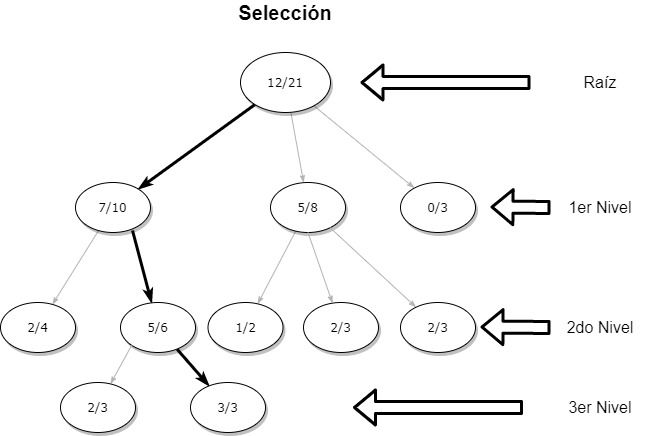
\includegraphics[width=0.5\textwidth,height=\textheight]{./diagramas/seleccion.jpg}
\caption{Selección}
\end{figure}

\emph{Expansión:} empezar desde la raíz \emph{R} y seleccionar nodos
hijos sucesivos hasta alcanzar un nodo hoja \emph{L}. La selección
describe una manera de elegir los nodos hijos, que permitan que el árbol
se expanda hacia movimientos mas prometedores, que es la esencia del
árbol de búsqueda Monte Carlo.

\begin{figure}
\centering
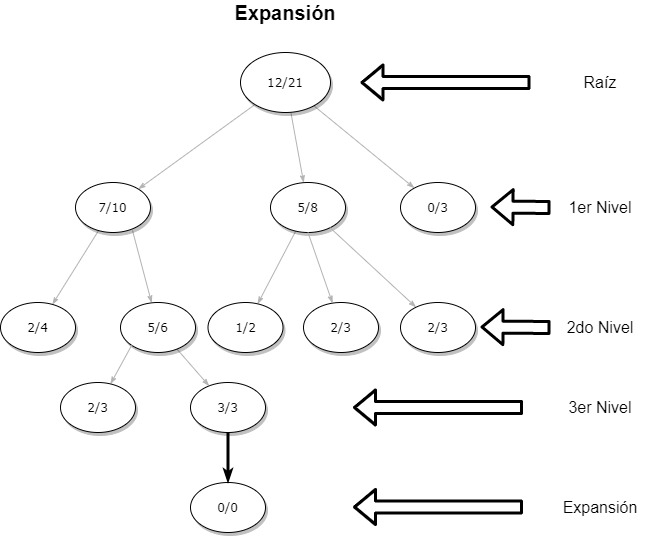
\includegraphics[width=0.5\textwidth,height=\textheight]{./diagramas/expansion.jpg}
\caption{Expansión}
\end{figure}

\newpage

\emph{Simulación:} realizar una simulación aleatoria desde el nodo C.

\begin{figure}
\centering
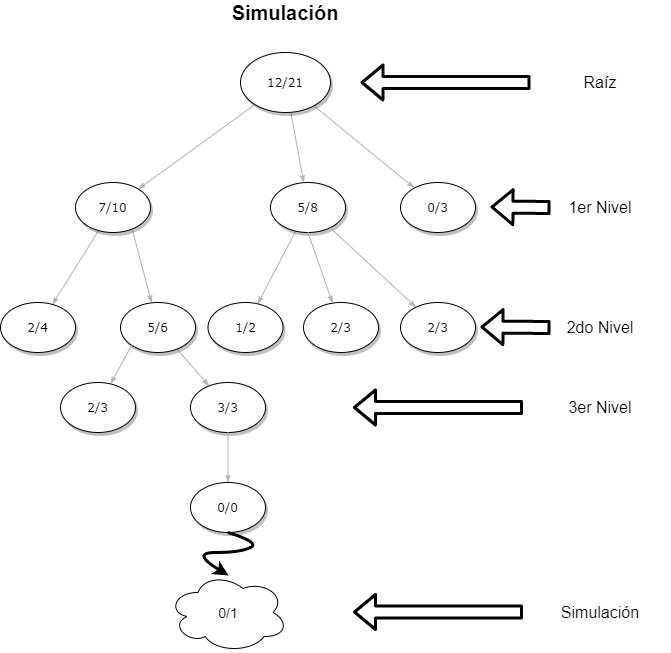
\includegraphics[width=0.5\textwidth,height=\textheight]{./diagramas/simulacion.jpg}
\caption{Simulación}
\end{figure}

\emph{Retro Propagación:} utilizar el resultado de la simulación para
actualizar la información en los nodos en el camino de \emph{C} a
\emph{R}.

\begin{figure}
\centering
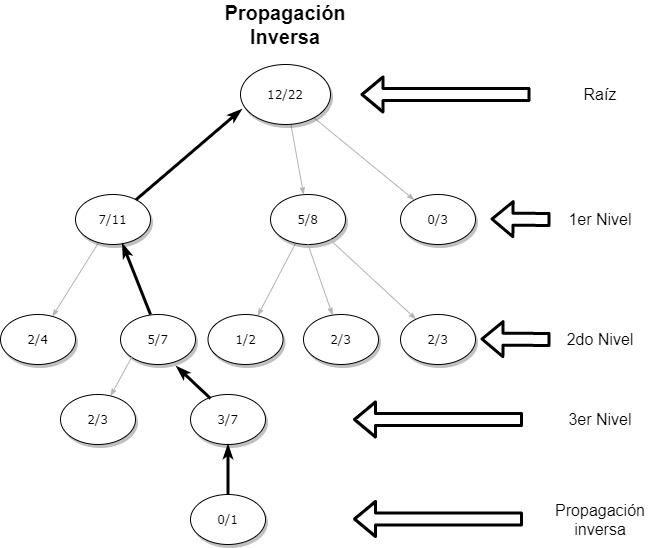
\includegraphics[width=0.5\textwidth,height=\textheight]{./diagramas/backpropagation.jpg}
\caption{Retro Propagación}
\end{figure}

\newpage

\hypertarget{codificaciuxf3n}{%
\subsubsection{Codificación}\label{codificaciuxf3n}}

La codificación de Búsqueda Monte Carlo es relativamente sencilla, al
hacer uso de el método de búsqueda ciega:

\begin{Shaded}
\begin{Highlighting}[]
\NormalTok{mcsearch}
\end{Highlighting}
\end{Shaded}

\begin{verbatim}
## function (N, lower, upper, Fx, type = "min", ...) 
## {
##     D <- length(lower)
##     s <- matrix(nrow = N, ncol = D)
##     for (i in 1:N) s[i, ] = runif(D, lower, upper)
##     fsearch(sol = s, Fx = Fx, type = type, ...)
## }
\end{verbatim}

Su implementación de igual manera es sencilla:

\begin{Shaded}
\begin{Highlighting}[]
\NormalTok{N=}\DecValTok{10000} \CommentTok{# se define el número de muestras}
\CommentTok{#para la función de esfera:}
\NormalTok{D <-}\StringTok{ }\KeywordTok{c}\NormalTok{(}\DecValTok{2}\NormalTok{,}\DecValTok{30}\NormalTok{)}
\NormalTok{label=}\StringTok{"esfera"}
\ControlFlowTok{for}\NormalTok{(i }\ControlFlowTok{in} \DecValTok{1}\OperatorTok{:}\KeywordTok{length}\NormalTok{(D))}
\NormalTok{\{ }
\NormalTok{  S=}\KeywordTok{mcsearch}\NormalTok{(N,}\KeywordTok{rep}\NormalTok{(}\OperatorTok{-}\FloatTok{5.2}\NormalTok{,D[i]),}\KeywordTok{rep}\NormalTok{(}\FloatTok{5.2}\NormalTok{,D[i]),sphere,}\StringTok{"min"}\NormalTok{)}
  \KeywordTok{cat}\NormalTok{(label,}\StringTok{"D:"}\NormalTok{,D[i],}\StringTok{"s:"}\NormalTok{,S}\OperatorTok{$}\NormalTok{sol,}\StringTok{"f:"}\NormalTok{,S}\OperatorTok{$}\NormalTok{eval,}\StringTok{"}\CharTok{\textbackslash{}n}\StringTok{"}\NormalTok{)}
\NormalTok{\}}
\end{Highlighting}
\end{Shaded}

\begin{verbatim}
## esfera D: 2 s: -0.02428153 f: 0.003577936 
## esfera D: 30 s: -0.6641743 f: 108.1639
\end{verbatim}

\begin{Shaded}
\begin{Highlighting}[]
\NormalTok{label=}\StringTok{"Rastrigin"}
\ControlFlowTok{for}\NormalTok{(i }\ControlFlowTok{in} \DecValTok{1}\OperatorTok{:}\KeywordTok{length}\NormalTok{(D))}
\NormalTok{\{ S=}\KeywordTok{mcsearch}\NormalTok{(N,}\KeywordTok{rep}\NormalTok{(}\OperatorTok{-}\FloatTok{5.2}\NormalTok{,D[i]),}\KeywordTok{rep}\NormalTok{(}\FloatTok{5.2}\NormalTok{,D[i]),rastrigin,}\StringTok{"min"}\NormalTok{)}
\KeywordTok{cat}\NormalTok{(label,}\StringTok{"D:"}\NormalTok{,D[i],}\StringTok{"s:"}\NormalTok{,S}\OperatorTok{$}\NormalTok{sol,}\StringTok{"f:"}\NormalTok{,S}\OperatorTok{$}\NormalTok{eval,}\StringTok{"}\CharTok{\textbackslash{}n}\StringTok{"}\NormalTok{)}
\NormalTok{\}}
\end{Highlighting}
\end{Shaded}

\begin{verbatim}
## Rastrigin D: 2 s: -0.003405824 f: 0.04997579 
## Rastrigin D: 30 s: -2.882636 f: 356.9194
\end{verbatim}

\newpage
\singlespacing 
\end{document}